\iffalse
\let\negmedspace\undefined
\let\negthickspace\undefined
\documentclass[journal,12pt,twocolumn]{IEEEtran}
\usepackage{cite}
\usepackage{amsmath,amssymb,amsfonts,amsthm}
\usepackage{algorithmic}
\usepackage{graphicx}
\usepackage{textcomp}
\usepackage{xcolor}
\usepackage{txfonts}
\usepackage{listings}
\usepackage{enumitem}
\usepackage{mathtools}
\usepackage{gensymb}
\usepackage{comment}
\usepackage[breaklinks=true]{hyperref}
\usepackage{tkz-euclide}
\usepackage{listings}
\usepackage{gvv}
\def\inputGnumericTable{}
\usepackage[latin1]{inputenc}
\usepackage{color}
\usepackage{array}
\usepackage{longtable}
\usepackage{calc}
\usepackage{multirow}
\usepackage{hhline}
\usepackage{ifthen}
\usepackage{lscape}

\newtheorem{theorem}{Theorem}[section]
\newtheorem{problem}{Problem}
\newtheorem{proposition}{Proposition}[section]
\newtheorem{lemma}{Lemma}[section]
\newtheorem{corollary}[theorem]{Corollary}
\newtheorem{example}{Example}[section]
\newtheorem{definition}[problem]{Definition}
\newcommand{\BEQA}{\begin{eqnarray}}
\newcommand{\EEQA}{\end{eqnarray}}
\newcommand{\define}{\stackrel{\triangle}{=}}
\theoremstyle{remark}
\newtheorem{rem}{Remark}
\begin{document}

\bibliographystyle{IEEEtran}
\vspace{3cm}

\title{GATE 2023 BM 30}
\author{EE23BTECH11007 - Aneesh Kadiyala$^{*}$% <-this % stops a space
}
\maketitle
\newpage
\bigskip

\renewcommand{\thefigure}{\theenumi}
\renewcommand{\thetable}{\theenumi}

\vspace{3cm}
\textbf{Question:} In the following circuit, the switch S is open for $t < 0$ and closed for $t \ge 0$.
What is the steady state voltage (in Volts) across the capacitor when the switch is closed?
\begin{figure}[h!]
    \centering
    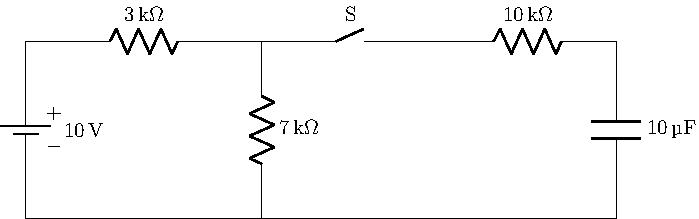
\includegraphics[width = \columnwidth]{2023/BM/30/figs/c_fig1.pdf}
\end{figure}
\\
\solution
\\
\fi
\begin{figure}[h!]
    \centering
    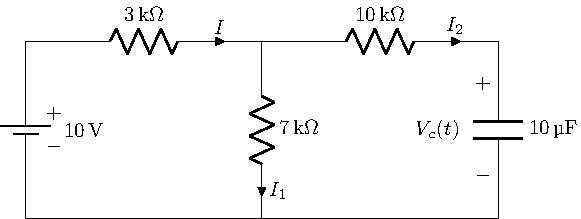
\includegraphics[width=\columnwidth]{2023/BM/30/figs/c_fig3.pdf}
\end{figure}
\\
In steady state, no current flows through the capacitor.
\begin{align}
I_2 &= 0 \\
V_c &= \brak{7\text{k}\ohm}I_1 \\
&= \brak{7\text{k}\ohm}I \\
&= \brak{7\text{k}\ohm}\frac{10\text{V}}{10\text{k}\ohm} \\
\implies V_c &= 7\text{V}
\end{align}
In s-domain:
\begin{figure}[h!]
    \centering
    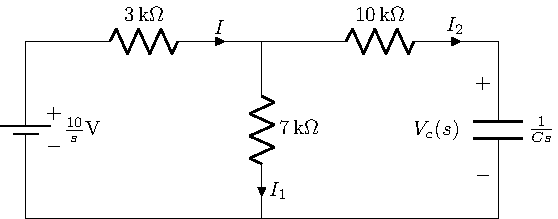
\includegraphics[width=\columnwidth]{2023/BM/30/figs/c_fig2.pdf}
\end{figure}
\begin{align}
\implies I\brak{s} &= \frac{\frac{10}{s}\text{V}}{3\text{k}\ohm + \frac{(7\text{k}\ohm)(10\text{k}\ohm + \frac{1}{sC})}{17\text{k}\ohm + \frac{1}{sC}}} \\
I &= I_1 + I_2 \\
I_1\brak{7\text{k}\ohm} &= I_2\brak{10\text{k}\ohm + \frac{1}{sC}} \\
I_2\brak{s} &= \frac{7\text{k}\ohm}{17\text{k}\ohm + \frac{1}{sC}}I\brak{s} \\
%&= \frac{\frac{70000}{s}}{121 * 10^6 + \frac{10000}{sC}} \\
%&= \frac{\frac{7}{s}}{121 * 10^2 + \frac{1}{sC}} \\
\implies I_2\brak{s} &= \frac{7\brak{10^{-5}}}{0.121s + 1} \\
V_c\brak{s} &= I_2\brak{s}\frac{1}{sC} \\
&= \frac{7}{s\brak{0.121s + 1}} \\
%&= 7\brak{\frac{\frac{1}{0.121}}{s\brak{s + \frac{1}{0.121}}}} \\
&= 7\brak{\frac{1}{s} - \frac{1}{s + \frac{1}{0.121}}}
\end{align}
Taking inverse Laplace transform:
\begin{align}
V_c\brak{t} &= 7u\brak{t}\brak{1 - e^{-\frac{t}{-0.121}}} \label{eq:2023BM30}
\end{align}
\begin{figure}[h!]
\centering
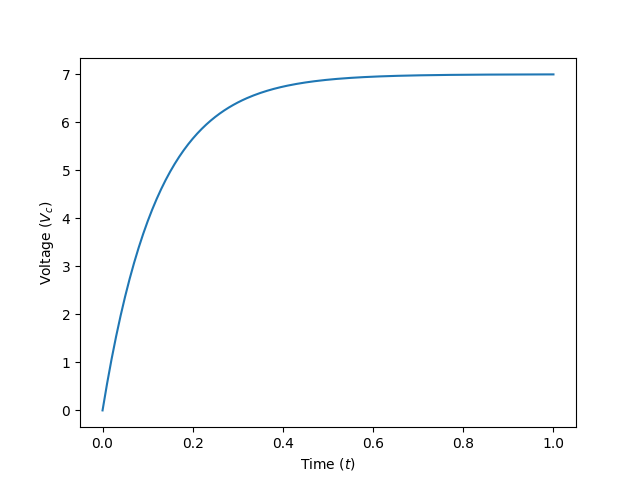
\includegraphics[width=\columnwidth]{2023/BM/30/figs/plot.png}
%\caption{$V_c$ vs $t$}
\label{fig:2023BM30}
\end{figure}
\\
In steady state $t \to \infty$. From \eqref{eq:2023BM30}:
\begin{align}
\lim_{t\to\infty}V_c\brak{t} &= 7\text{V}
\end{align}
